\chapter{Założenia metodologiczne}

W poniższym rozdziale przedstawię elementy składowe jakie stanowiły części wykonanych eksperymentów.

\section{Wybrane zbiory danych}

W pracy posłużyłem się dwoma zbiorami danych:
\begin{itemize}
	\item Casia image tampering detection evaluation database \cite{casia}
	\item The PS-Battles Dataset \cite{ps}
\end{itemize}

\subsection{CASIA v.2}

Opisywany zbiór posiada $12 614$ zdjęć, z czego $7 941$ z nich stanowi zdjęcia oryginalne, a kolejne $5 123$ to zdjęcia zmanipulowane(patrz rysunek \ref{fig:casia} ). Zgodnie z artykułem \cite{casia} elementy zbioru różnią się wielkością od $320 \times 240$, aż do $800 \times 600$ pikseli. Manipulacja zdjęć jest wykonana poprzez wycinanie, kopiowanie i rozmazanie. Twórcy zbioru danych podzielili go na $9$ kategorii: scena, zwierzę, architektura, postać, roślina, artykuł, natura, wnętrze i tekstura - na potrzeby pracy interesuje Nas tylko podział na dane prawdziwe i zmanipulowane. Dodatkowo zdjęcia zawarte w zbiorze zapisane są jako *.JPEG, *.BMP, *.TIFF.

\begin{figure}[h!]
	\includegraphics[width=7cm]{casia.png}
	\centering
	\caption{Ilość przedstawicieli danej klasy w zbiorze CASIA v.2}
	\label{fig:casia}
\end{figure}

\subsection{The PS-Battles Dataset}

Powyższy zbiór jest liczniejszy - $21 758$ elementów, z czego po $10 879$ należy do każdej z dwóch klas(patrz rysunek \ref{fig:ps}). Formatem zdjęć jest *.JPEG lub *.PNG, a wielkość jest różna od $136 \times 68$, do aż $20 000 \times 12 024$ pikseli. Zbiór danych został stworzony przez społeczność forum internetowego \textit{reddit.com/r/photoshopbattles} do której na moment pisania pracy należy $\sim16,5$ mln użytkowników, którzy to codziennie dodają kolejne $\sim92$ posty ze zdjęciami. Ideą tej społeczności jest wrzucanie zdjęć nieoczywistych, śmiesznych a następnie przerabianie ich na śmieszniejsze.

\begin{figure}[h!]
	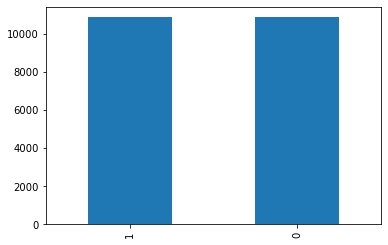
\includegraphics[width=7cm]{ps.png}
	\centering
	\caption{Ilość przedstawicieli danej klasy w zbiorze PS-Battles}
	\label{fig:ps}
\end{figure}

\section{Stratyfikowana k-krotna walidacja krzyżowa}

Do przeprowadzenia wiarygodnych eksperymentów i wyliczeniu odpowiednich metryk pracy modeli skorzystałem z k-krotnej stratyfikowanej walidacji krzyżowej. W samej k-krotnej walidacji krzyżowej chodzi po prostu o podział zbioru $Z$ na $k$ równych elementów \cite{hands_on}. Następnie $1$ z tych $k$ zbiorów zostaje zbiorem testowym $Z_{t}$ podczas gdy pozostałe $k-1$ zbiorów zostają zbiorem uczącym $Z_u$. Całe zadanie jest powtarzane $k$ razy. Całość została pokazana na rysunku \ref{fig:walidacja}

\begin{figure}[h!]
	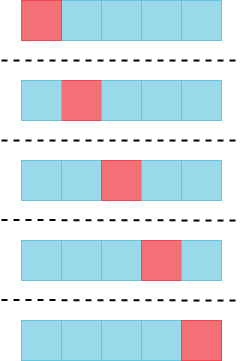
\includegraphics[width=5cm]{walidacja.png}
	\centering
	\caption{Przebieg 5-krotnej walidacji krzyżowej}
	\label{fig:walidacja}
\end{figure}

Z racji jednak że w zbiorze testowym CASIA \cite{casia} ilość przedstawicieli klas nie jest taka sama - zdecydowałem się na stratyfikowaną wersję k-krotnej walidacji krzyżowej, oznacza to że podczas podziału na podzbiory operacja ta zachowuje oryginalny lub zbliżony do oryginalnego poziom niezbalansowania danych.

\section{Parowe testy statystyczne}

Do sprawdzenia czy po przeprowadzeniu eksperymentu na tych samych modelach ale np. różnych jądrach, różnice które otrzymałem w wartościach metryk są istotne statystycznie, skorzystałem z testu \textit{T-Studenta} z poziomem ufności $\alpha = 0,05$ \cite{stata}. Obliczenia zostały przeprowadzone dla każdej z metryk, tj. dokładności, czułości, precyzji i miary \textit{F}. Za hipotezę zerową przyjąłem, że pomiędzy klasyfikatorami nie ma istotnej różnicy statystycznej, co oznacza że kiedy wyliczona przez statystykę $t$, wartość $p-value$ będzie mniejsza lub równa $\alpha$ - odrzucę hipotezę zerową. W przeciwnym wypadku($\alpha>p-value$) przyjmę hipotezę zerową.

\section{Maszyna wektorów nośnych(\textit{SVM})}

Jako bazowym klasyfikatorem binarnym posłużyłem się maszyną wektorów nośnych(ang. \textit{Support Vector Machine} - \textit{SVM}). Ideą tego algorytmu jest rzutowanie danej przestrzeni cech, na przestrzeń o większej ilości wymiarów. Taka operacja pozwala osiągnąć własność zwaną liniową separowalnością. Oznacza to nie mniej ni więcej, że istnieje możliwość rozdzielenia zbioru uczącego, tj. ${(\vec{x}_{1},y_{1}),...,(\vec{x}_{n},y_{n})}$ za pomocą hiperpłaszczyzny separującej, opisanej wzorem \ref{eqn:svm}
\begin{equation}
	\vec{w} * \vec{x}-b=0
	\label{eqn:svm}
\end{equation}
, gdzie $\vec{w}$ jest wektorem normalnym dla tej płaszczyzny. Ponadto, wyliczane są wektory nośne, takie żeby spełniały własność opisaną wzorem \ref{eqn:supp}
\begin{equation}
	\begin{split}
		\vec{w} * \vec{x}-b &=1 \\
		\vec{w} * \vec{x}-b &=-1
	\end{split}
	\label{eqn:supp}
\end{equation}
Tym samym poszczególne próbki są rozdzielane ponad lub poniżej hiperpłaszczyzny separującej, co zostało zobrazowane na rysunku \ref{fig:svm}.
\begin{figure}[h!]
	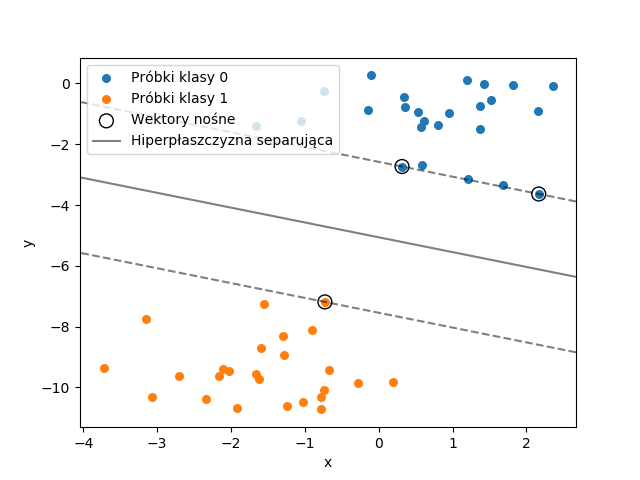
\includegraphics[width=10cm]{svm.png}
	\centering
	\caption{Przykład klasyfikacji maszyny wektorów nośnych}
	\label{fig:svm}
\end{figure}

\section{Analiza głównych składowych}

Dla uczącego zbioru danych $Z_{u}$, składającego się z $n$ obserwacji, gdzie każda ma postać ${k_{1}, ..., k_{i}}$ można zdefiniować chmurę punktów, która im odpowiada. Oczywiście, mamy wtedy do czynienia z $n$ punktów w przestrzeni $i$ wymiarowej \cite{pca}. Na potrzeby przykładu można przyjąć że mamy do czynienia z $n=50$ i $i=2$. Celem analiza głównych składowych(z ang.\textit{principal component analysis}- \textit{PCA}) jest taki obrót układu współrzędnych, aby maksymalizować wartość wariancji pierwszej współrzędnej, a następnie drugiej. Obrót ten, ma na celu skonstruowanie nowej przestrzeni, w której to początkowe współrzędne są najważniejsze. Graficzny przykład omawianej operacji widoczny jest na rysunku \ref{fig:pca}.

\begin{figure}[h!]
	\centering
	\subfloat{{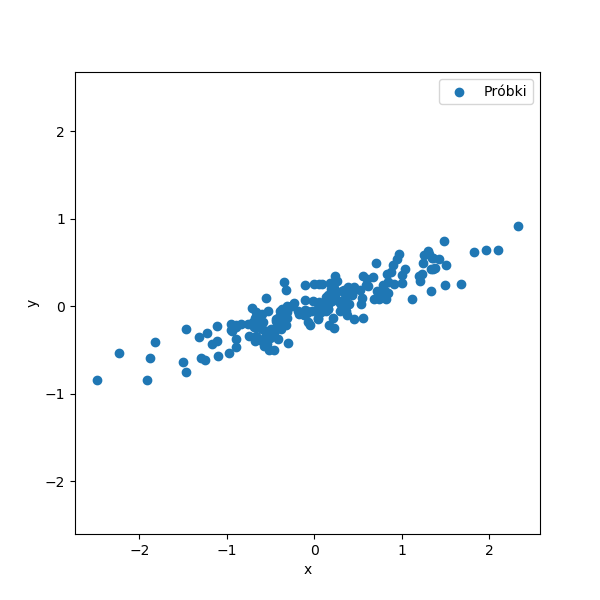
\includegraphics[width=6cm]{data_PCA.png} }}
	\qquad
	\subfloat{{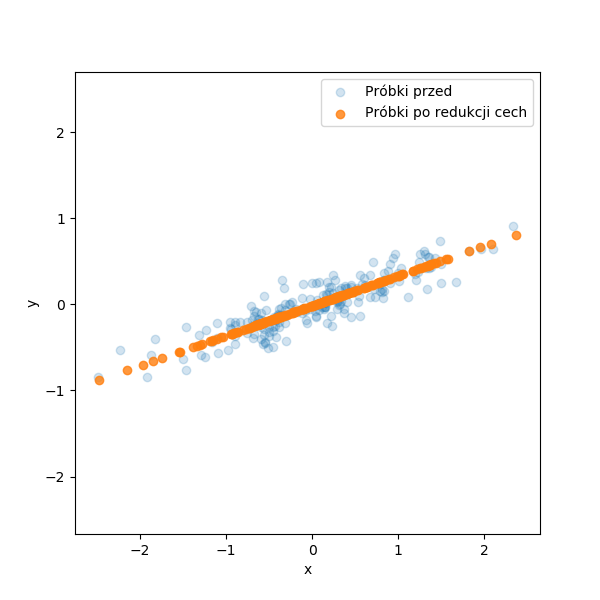
\includegraphics[width=6cm]{after_PCA.png} }}
	\caption{Dane przed i po redukcji cech przy pomocy PCA(n\_components=1)}
	\label{fig:pca}
\end{figure}

\section{VGG Net}

Architektura splotowej sieci neuronowej VGG Net została zaproponowana na przełomie 2014 i 2015 roku, przez K.  Simonyan i A. Zisserman \cite{vgg}. Wykorzystywała ona 19 warstw oraz bardzo małe jak na te czasy filtry splotowe($3 \times 3$). Sam skok splotu, jak i jego wypełnienie(z ang. \textit{padding}) wynosiło 1 piksel. Takie potraktowanie danych pozwoliło uzyskać mapy aktywacji posiadające takie same rozdzielczości co na wejściach warstw splotowych. Zabieg ten spowodował że wydłużanie łańcucha takich połączeń stało się bardzo proste. \\

Ważnym punktem tej architektury i towarzyszącej jej pracy naukowej \cite{vgg} jest zauważenie przez autorów że moduł składający się z 3 warstw $3 \times 3$ ma efektywne pole postrzegania takie jak pojedyncza warstwa $7 \times 7$., przy używaniu dużo mniejszej liczby parametrów praz używaniu trzech nieliniowości zamiast jednej. Wniosek ten sprawił że w dalszych pracach w dziedzinie można zauważyć ewidentne zwrócenie się w stronę wykorzystywania większej ilości warstw z coraz mniejszymi wielkościami filtrów.
